
\documentclass[a4paper,12pt]{article}

\usepackage{amsmath}
\usepackage{amssymb}
\usepackage{mathrsfs}
\usepackage{blindtext}
\usepackage{float}
\usepackage{multicol}
\usepackage{graphicx}
\usepackage{cmap}					% поиск в PDF
\usepackage[T2A]{fontenc}			% кодировка
\usepackage[utf8]{inputenc}			% кодировка исходного текста
\usepackage[english,russian]{babel}	% локализация и переносы
\usepackage{geometry}
\usepackage{graphicx}
\usepackage{tikz} 
\usepackage{pgfplots}

\usepackage{xcolor}
\usepackage{listings}
\lstset{basicstyle=\ttfamily,
  showstringspaces=false,
  commentstyle=\color{red},
  keywordstyle=\color{blue}
}

\addto\captionsrussian{\def\refname{}}

\linespread{1.3} % полуторный интервал
\frenchspacing

\begin{document}

\begin{center}
    \textbf{Аннотация}
\end{center}

\begin{center}
    Сравнение on-disk алгоритмов поиска подстроки в строке
\end{center}

В современном мире существуют задачи анализа большого количество данных. В число таких задач входит поиск подстроки в строке в тексте, последовательностях ДНК или последовательностях белков. Для эффективного не только по времени, но и по занимаемому пространству, поиска используются сжатые индексы, которые предполагают, что текст и сам индекс находятся в RAM. Однако, при большом количестве данных, когда ни текст, ни индекс текста не помещаются в оперативную память, используются специализированные для дисков структуры данных, которые учитывают особенности ввода-вывода блочных устройств. Комбинация сжатых и блочных структур данных позволяет добиться эффективного поиска по тексту во внешней памяти, а также не занимать много места на диске.

В данной работе исследуются, реализуются и сравниваются две структуры данных: String B-Tree и String B-Tree + Geometric Burrows-Wheeler Transform. Их отличие заключается в том, что вторая реализуется на основе первой, но при этом занимает меньше места за счёт сжатых индексов. Были получены результаты, что сжатая структура занимает на диске в 4 раза меньше места по сравнению с обычной, однако работает в два раза дольше.

\newpage

\begin{center}
    \textbf{Обозначения, сокращения и определения}
\end{center}

\noindent
\textbf{SA} - \textit{Suffix array} - структура данных суффиксный массив.\newline
\textbf{BT} - \textit{B-Tree} - структура данных B-Tree - сильно ветвистое дерево поиска.\newline
\textbf{SBT} - \textit{String B-Tree} - структура данных дерево поиска, основанное на B-Tree.\newline
\textbf{ДНК} - \textit{Дезоксирибонуклеиновая кислота} - последовательность из азотистых основание A,C,T,G.\newline
\textbf{I/O} - \textit{Input / Output} - операции ввода-вывода внешнего устройства \newline
\textbf{gcc} - \textit{GNU Compiler Collection} - набор компиляторов для различных языков программирования, разработанный в рамках проекта GNU.\newline
\textbf{ОЗУ} - \textit{Оперативное запоминающее устройство } - оперативная память. \newline
\textbf{RAM} - \textit{ Random Access Memory } - ОЗУ подчёркивая, что время обращения в случайные области невелико. \newline
\textbf{$\mu s$} - микросекунда. \newline
\textbf{MB} - \textit{Mega Byte} - 1024 * 1024 Байт. \newline

\newpage

\tableofcontents

\newpage

\section{Введение}

\textbf{Актуальность темы исследования.} В современном мире количество цифровой информации постоянно растёт, а потребность их анализировать не спадает. В частоности, существует задача анализа больших последовательностей данных, которая встречается в таких областях как биоинформатика. Размер исследуемых данных в этой области может сильно варьироваться и занимать от 500 Мбайт до 3 Гбайт данных для последовательности ДНК человека или Бета-варианта коронавируса \cite{BLAST} или же сотни гигабайт для наборов геномов людей в целях исследования различных болезней \cite{1000HumanGenom}. Однако даже самый современный персональный компьютер на базе процессора Apple M2 Ultra\cite{Apple192Gb}, который в максимальной комплектации имеет 192 Гбайта оперативной памяти и 8 Тбайт SSD, не сможет хранить данные из второго примера у себя в ОЗУ, однако в 90 раз больший объём диска позволит разместить их на диске. Такая тенденция, что размер диска на порядки больше, чем размер ОЗУ, является следствием развития текущих технологий и встречается во всех персональных компьютерах. В связи с чем остро встаёт вопрос анализа последовательностей данных во внешней памяти с учётом свойств SSD дисков \cite{cobb2012nvm} \cite{agrawal2008design} эффективного не только по времени, но и занимаемому пространству на диске. Для таких задач используются специальные сжатые индексы для дисков, которые позволяют максимально экономно использовать память, не теряя при эффективных свойств поисковых операций. Одной из базовых и важных задач анализа последовательностей данных является поиск подстроки в строке, который и будет рассмотрен в этой работе.

\textbf{Цели и задачи работы.} Целью данной работы является сравнение времени поиска и занимаемого пространства на диске двух струткрур данных в задаче поиска подстроки $P$ в строке $T$ во внешней памяти: 
\begin{itemize}
    \item String B-Tree - on-disk структура поиска по тексту
    \item Geometric BWT - on-disk структура поиска по тексту со сжатыми индексами
\end{itemize}

Для достижения поставленной цели ставятся следующие задачи исследования:
\begin{enumerate}
    \item Исследовать существующие сжатые индексы \cite{gonzalez2007compressed}\cite{navarro2007compressed}\cite{mishra2018fast}
    \item Исследовать существующие струткры данных $SBT$ и $GBWT$ \cite{chien2008geometric}\cite{culpepper2010top}\cite{ferragina1999string}\cite{chiu2010efficient}
    \item Реализовать структуры данных на языке C++20 \cite{вандервуд2003шаблоны}
    \item Провести эксперимент при различных параметрах структур и длинах текстах для получения подтверждения меньшего размера сжатых структур, по сравнению с обычными, а также получения времени поиска.
\end{enumerate}

\textbf{Практическая значимость.} Полученные в работе результаты могут быть использованы в приложениях  обработки сигналов, анализе генетических кодов и последовательностей белков, обработки больших объёмов текстовой информации и во всех прикладных задачах, где требуется поиск подстроки в строке, и размер входных данных гораздо больше оперативной памяти устройства.

\newpage

\section{Обзор известных методов}
\subsection{Задача поиска подстроки в строке и индекс}
Перед тем как переходить к комплексным структурам данных поиска на внешних устройствах и сравнению их производительности, необходимо последовательно определить задачу поиска, рассмотреть базовые структуры данных, которые будут использоваться как строительные блоки, а также отметить фундаментальные идеи используемых алгоритмов поиска.

Под задачей поиска подстроки в строке в данной работе будет подразумеваться поиск позиции первого вхождения паттерна $P[0, p-1]$ в тексте $T[0, n-1]$. Размер алфавита будет обозначаться символом $\sigma$. К примеру, при рассмотрении последовательности ДНК, которая состоит из азотистых оснований $A,C,T,G$, размер алфавита $\sigma = 4$. В работе часто будет использоваться логарифм по основанию $2$, поэтому основание будет опускаться, и записываться как $\log\sigma$.

Существует много эффективных способов решить эту задачу в оперативной памяти, например, построение сжатого суффиксного дерева (компактный бор) или суффиксного массива, но сейчас будет рассмотрен суффиксный массив (\textit{Suffix Array, сокращённо SA}) и преобразование Берроуза-Уилера (\textit{Burrows–Wheeler transform, сокращённо BWT}).

\subsubsection{Суффиксный массив}
Рассмторим текст $T[0, n-1]$ построенный над алфавитом размера $\sigma$. Введём обозначение суффикса $T[i, n-1]$, где $i=0,..,n-1$, тогда у текста существует ровно $n$ суффиксов, которые можно однозначно задать, указав позицию его начала в тексте $i$. Отсортируем суффиксы в лексикографическом порядке и запишем их позиции в массив размера $n$. Полученный массив чисел называется суффиксным массивом, его размер составляет $n\log{n}$ бит.

Ниже приведена иллюстрация суффиксного массива из статьи G. Navarro and V. Mäkinen \cite{navarro2007compressed}:

\begin{figure}[h!]
\center{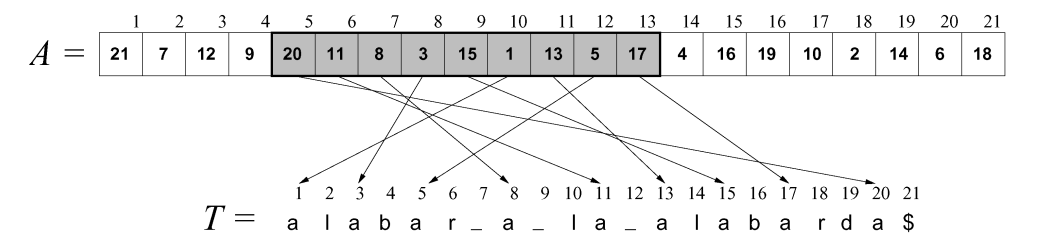
\includegraphics[width=170mm]{images/SA.png}}
\caption{Суффиксный массив над текстом T = "alabar a la alabarda"}
\end{figure}

У этой структуры данных есть полезное свойство: если было найдено, что паттерн $P$ начинает встречаться c позиции $i$, то все остальные суффиксы, которые начинаются с этого паттерна, идут сразу с позиции $i+1$, либо же он больше не встречается. 
При помощи суффиксного массива, можно выполнять поиск подстроки в строке, делая бинарный поиск по отсортированному массиву строк, он приведён на Рис. 2 (G. Navarro and V. Mäkinen \cite{navarro2007compressed}).

\begin{figure}[h!]
\center{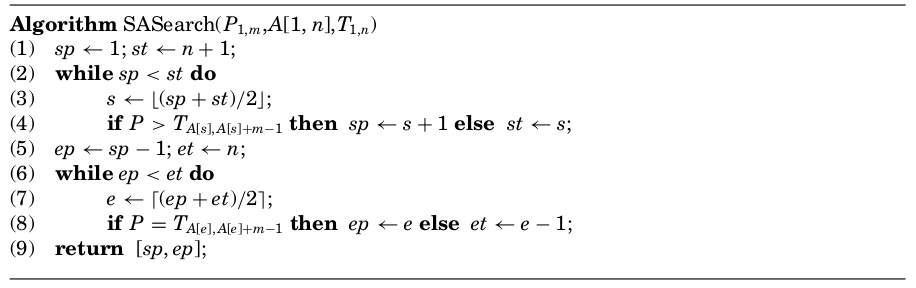
\includegraphics[width=170mm]{images/SA_Search.png}}
\caption{Алгоритм поиска паттерна $P$ в тексте $T$ при помощи суффиксного массива}
\end{figure}

\subsubsection{BWT. Преобразование Берроуза-Уилера}
Преобразование Берроуза-Уиллера над текстом $T[0, n-1]$ можно получить следующим образом. Без уменьшения общности добавим нулевой завершающий символ, который меньше всех символов из алфавита текста и исторически обозначается как $\$$,. При помощи циклического сдвига строки, получим все суффиксы текста $T$ с точностью до завершающего символа, а затем запишем их сверху внизу, чтобы получить матрицу. Далее отсортируем эти строки. В получившейся матрице $M$ первый столбец очевидно будет представлять из себя суффиксный массив исходного текста, а последний столбец как раз и представляет из себя последовательность $T^{BWT}$. Более строго, преобразование $BWT$ над текстом $T$ - это $T^{BWT}[i]=T[SA[i] - 1]$, где $SA$ - суффиксный массив $T$. По умолчанию принимается, что при $i$ таком, что $SA[i] = 0$, $T^{BWT}[i]=\$$

Более наглядно этот способ построения $T^{BWT}$ приведён на Рис.3 (G. Navarro and V. Mäkinen \cite{navarro2007compressed}).

\begin{figure}[h!]
\center{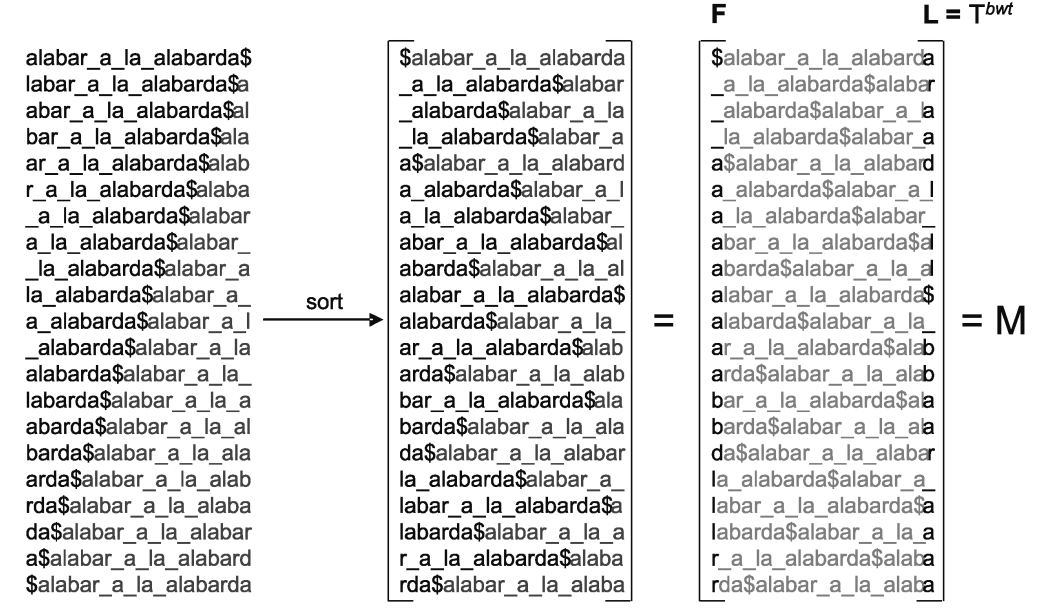
\includegraphics[width=160mm]{images/BWT.png}}
\caption{Построение $T^{BWT}$ над $T$. В полученной матрице $M$ последний стобец $L = T^{BWT}$}
\end{figure}

Массив $T^{BWT}$ требует всего $nlog\sigma$ бит, что в сравнении с суффиксным массивом ($n\log{n}$ бит) при больших текстах сильно меньше. Преобразование $BWT$ используется в так называемом обратном поиске или же \textit{Backward Search}. Суть его в том, что поиск позиции вхождения паттерна $P$ в текст $T$ начинается не с начала паттерна, а с его конца.

\subsubsection{Обратный поиск. Backward Search}
Одна из важных идей, которая пригодится в работе в дальнейшем, - это обратный поиск \cite{grabowski2017fm} паттерна в тексте, который использует $T^{BWT}$, полученный после преобразования Берроуза-Уилера, а также вспомогательный массив $C$. Массив $C$ имеет размер $\sigma$ и строится следующим образом: пусть текст состоит из чисел от 0 до $\sigma-1$, тогда в ячейку массива $C[i+1]$ положим количество встреч символа $i$ в тексте. Например, если символ $"2"$ встречается в тексте 5 раз, то $C[2]=5$. Затем ко второй ячейке прибавим первую, потом к третей прибавим вторую и так далее. Это и будет итоговый массив $C$.

Идея обратного поиска в том, что на каждом шаге ищется диапазон $[l,r]$ суффиксного массива, в котором должен быть суффикс паттерна. Поиск паттерна $P$ в тексте $T$ начинается с последнего символа паттерна. Первый диапазон, в котором все суффиксы текста начинаются с последнего символа паттерна, находится элементарно - это элемент $[C[x], C[x+1]]$, где $x$ - последний символ паттерна. Для следующих итераций нужно ввести операцию ранка над массивом $T^{BWT}$.

$rank_{T^{BWT}}(p, c)$ - это количество встреч символа $c$ в тексте $T^{BWT}$ до позиции $p$. Рассмотрим эту операцию на примере текста $T^{BWT}="ababbb"$, тогда $rank(2, a)=1$.

Второй и последующие интервалы получаются следующим образом: пусть предыдущий интервал $[sp_0, ep_0]$, тогда
\begin{align*}
sp_1 & = C['c'] + rank(sp_0, 'c')\\
ep_1 & = C['c'] + rank(sp_0 + 1, 'c') - 1
\end{align*}

После количества итераций равных размеру паттерна, получается интервал суффиксного массива, в котором лежат все вхождения паттерна. Данный алгоритм поиска хорошо и понятно проиллюстрирован на Рис.4 \cite{navarro2007compressed}, где текст T = "alabar a la alabarda", а паттерн P = "ala". Сначала для буквы 'a' получают диапазон $[5, 13]$, затем при рассмотрении буквы 'l', интервал меняется до $[17, 19]$, на первой букве 'a' получается итоговый интервал $[10,11]$. Для поиска необходим только массив $T^{BWT}$ и массив $C$, остальные элементы на рисунке показаны для наглядности.

\begin{figure}[h!]
\center{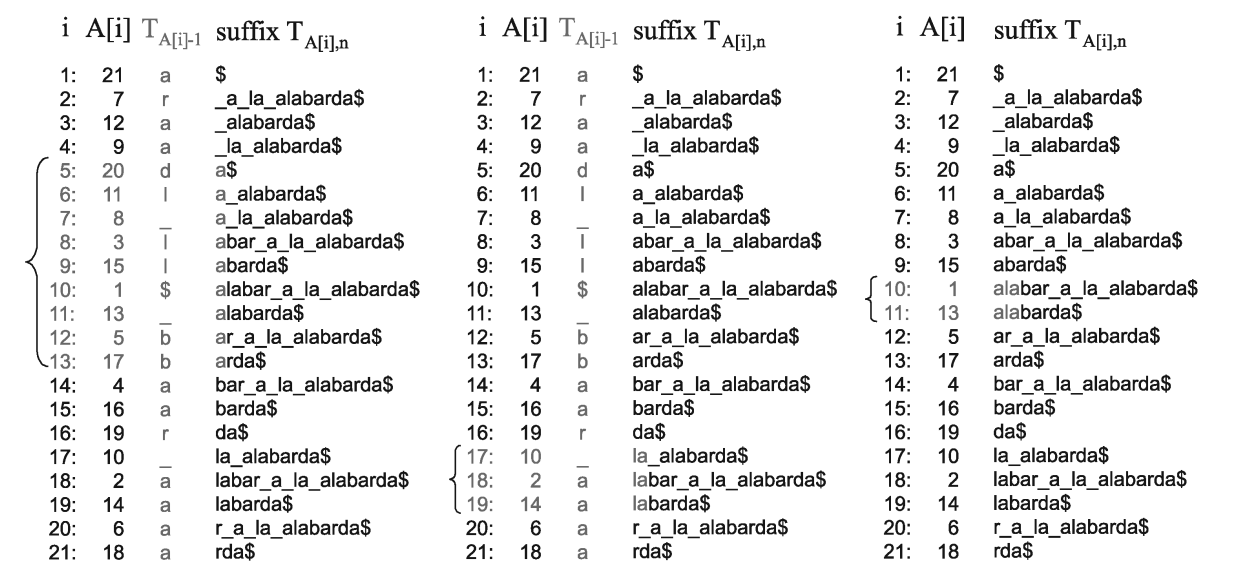
\includegraphics[width=160mm]{images/BackwardSearch.png}}
\caption{Алгоритм обратного поиска для текста T = "alabar a la alabarda" и паттерна P = "ala"}
\end{figure}

\subsection{Сжатые структуры данных}
\subsubsection{Введение}
Существует много различных структур данных с их полезными и эффективными свойствами, которые часто используются в своём первоначальном виде. Однако, может возникнуть ситуации, когда их размеры становятся недопустимо большими, например, когда дерево поиска разрастается настолько, что больше не может поместиться в оперативную память. В такой ситуации было бы очень полезно использовать структуру данных, которая бы работала также эффективно, как поисковое дерево из примера, но при этом занимала минимально возможное для этого место. Такие структуры данных есть и они называются сжатые. Сжатые структуры данных представляют из себя аналоги стандартных структур с тем ми же операциями, однако их размер существенно меньше, а эффективность либо примерно такая же, либо даже гораздо больше. Последнее зачастую возникает как следствие того, что структура начинает гораздо эффективнее пользоваться памятью и хорошо ложиться на кэш процессора, в итоге ему приходится анализировать меньше байт данных.

Следует однако уточнить, что сжатые структуры данных не представляют из себя аналог архива, который перед работой нужно полностью распаковать, такое поведение крайне неэффективно и более того не решает поставленную задачу уложиться в оперативную память. Сжатые структуры используют пространство максимально эффективно, они манипулируют буквально битами, чтобы достигнуть своей информационно-теоретической минимальной границы, при это сохранив эффективность первоначального алгоритма.

Самый простой и понятный пример такой сжатой структуры данных - это битовая карта или же битовый массив в inode, например, в файловой системе $Ext4$ \cite{mathur2007new}. Он позволяет очень быстро определить какие записи индексных дескрипторов заняты, а какие свободны.

Далее будут рассмотрены базовые сжатые структуры данных и их основополагающие операции над ними, которые в последствии будут использоваться для представления массива метасимволов, полученного после геометрического преобразования Берроуза-Уилера.

\subsubsection{Битовый вектор и базовые операции над сжатыми структурами}
Первое, с чего стоит начать рассмотрение сжатых структур данных, так это с базовых, однако фундаментальных операций над ними. Для начала рассмотрим битовый массив $B[0, n-1]$, элементами которого могут быть только числа $0$ либо $1$. Для битового массива базовые операции три:
\begin{enumerate}
    \item $get(i)$  - получить значение бита на позиции $i$
    \item $rank(pos)$ - получить количество единиц в битовом массиве до позиции $pos$ не включительно
    \item $select(index)$ - получить первую позицию $pos$ в битовом массиве, в которой $rank(pos)$ = index
\end{enumerate}

С операцией $get(i)$ всё очевидно, поэтому рассмотрим сразу операцию $rank$. Эта операция очень часто используется в алгоритмах над сжатыми структурами данных, её эффективная реализация за время доступа $O(1)$ будет описана ниже. Более общая запись для этой операции - $rank_1(pos)$. Также есть $rank_0(pos)$, которая считает количество нулей до позиции $pos$. Т.к. битовый массив состоит всего из нулей и единиц, то очевидно, что $rank_0(pos) = pos - rank_1(pos)$, где подразумевается, что $pos \in [0, n]$.

Операцию $select(index)$  лучше рассмотреть на примере. Пусть имеется битовый массив $B={1,0,1,0,1}$, тогда $select(0) = 0$, $select(1) = 2$, $select(2) = 4$. Это операция не такая тривиальная как $rank(pos)$, однако её тоже можно реализовать за константное время, что будет описано ниже. Операция $select$, также, как и $rank$, может быть и для нулей, тогда она обозначается как $select_0(index)$.

\subsubsection{Эффективная реализация операции $rank_b(pos)$}
Операция $rank_b(pos)$ используется очень часто, поэтому необходимо сделать эту операции эффективной. Самая простая реализация - непосредственно подсчёт строк не требует дополнительной памяти, однако занимает $O(n)$ времени. Чтобы выполнить запрос гораздо быстрее, а именно за $O(1)$ - константное время и при этом занять $o(n)$ дополнительной памяти, обратимся к реализации G. Navarro and V. Mäkinen \cite{navarro2007compressed}.

Для более удобной записи, будет использоваться сокращение $x/y$, которое эквивалентно делению по нижней границе: $\lfloor x/y \rfloor$. 

Идея быстрого выполнения операции $rank$ заключается в добавлении массивов, в которых хранятся предвычисленные ранки для определённых слоёв блоков. 

Начнём с самого верхнего слоя, а именно рассмотрим строку длиной $t=\frac{\log{n}}{2}$. Базовый подход заключается в том, чтобы сохранить всевозможные значения битовой строки длиной $t$, а именно $2^{t} = 2^{\frac{\log{n}}{2}} = \sqrt{n}$ значений, для всевозможных значений аргумента ранка такой строки $[0, t-1]$ в массиве $smallrank[0, \sqrt{n}-1][0, t-1]$, который будет занимать $\sqrt{n} * t * log(t) = \sqrt{n} * \frac{\log{n}}{2} * log\frac{\log{n}}{2} = o(n)$ дополнительной памяти. Такой массив позволяет за константное время определять значение ранка для данной строки следующим образом: $rank_1(smallblock, i) = smallrank[smallblock, i]$, где $smallblock$ - это текущая рассматриваемая строка длины $t$. Однако в современных реализациях такой массив не требуется, потому что значительное большинство современных процессоров имеют быструю функцию $popcount$, которая как раз и говорит сколько бит есть в числе (длина битовой строки $t=\frac{\log{n}}{2}$ даже для текста длиной $2^{64}$ символов будет $t=\frac{\log{2^{64}}}{2}=\frac{64}{2}=32$ бита, т.е это число). Стоит отметить, что если нужно получить ранк от строки, длиной $2t$, то достаточно выполнить операцию $rank$ сначала для одной половины, потом для другой и сложить их. В итоге, благодаря самому верхнему слою можно получить результат операции $rank_1$ для любой последовательности бит длиной $2t = \log{n}$ либо вообще не занимая дополнительной памяти, либо занимая $O(n)$ дополнительной памяти.

Следующий слой предполагает разбиение битового массива $B$ на блоки длиной $2t$ и хранении значения ранка на границе этих блоков в массиве \newline$sampledrank$. Однако, каждый результат занимает $\log{n}$ бит, что приводит к $\frac{n}{2t} \log{n} = \frac{n}{\log{n}}\log{n} = n \notin o(n)$ дополнительным занимаемым битам данных.

Чтобы решить проблему излишнего занимаемого места для слоя блоков, добавляется ещё один слой - слой суперблоков, а блоки хранят результат уже относительно суперблоков, а не начала массива. Размер суперблока $\log^2 n$. Массив из таких суперблоков хранит результат операции $rank(i \log^2 n)$, где $i \in [0, \frac{n}{\log^2 n}]$, размер ячейки $\log{n}$. Размер занимаемый всеми суперблоками будет равен $\frac{n}{\log^2 n}*\log n = \frac{n}{\log{n}} = o(n)$.

Блоки хранят значения в диапазоне $[0, \log^2{n}]$, поэтому элемент массива блока занимает $\log{\log^2{n}} = 2 \log \log n$, тогда в одном суперблоке все блоки занимают $\frac{\log^2{n}}{2t} = \frac{\log^2{n}}{\log{n}} = \log{n}$, что приводит к тому, что общая занимаемая дополнительная память для блоков составляет $\frac{n}{\log^2{n}} * \log{n} * 2 \log \log n = \frac{2n}{\log n} \log \log n = o(n)$.

Тем самым имея индекс $i$, для которого нужно выполнить $rank_1(i)$, результат определяется как сумма найденных значений в массиве суперблока, значения в блоке и двум значениям в $smallrank$ (либо $popcount$), что в итоге требует $O(1)$ операций и $O(n)$ дополнительной занимаемой памяти.
В качестве примера можно рассмотреть битовый массив $B={0, 1, 0, 1, 1, 0, 1, 0, 0, 1, 1, 1, 0, 1, 0, 0}$ и запрос $rank_1(11)$, иллюстрация вычисления такого ранка представлена на рис. 5.

Стоит отметить, что существует более ёмкая по памяти реализация $rank$ за константное время, которая представляет битовый массив как пары чисел и требует $nH_0 + o(n)$ бит памяти вместе с битовым массивом, где $H_0$ - энтропия нулевого порядка битового массива $B$. Однако такая реализация гораздо сложнее ложится на диск, поэтому в данной статье не рассматривается.

\begin{figure}[h!]
\center{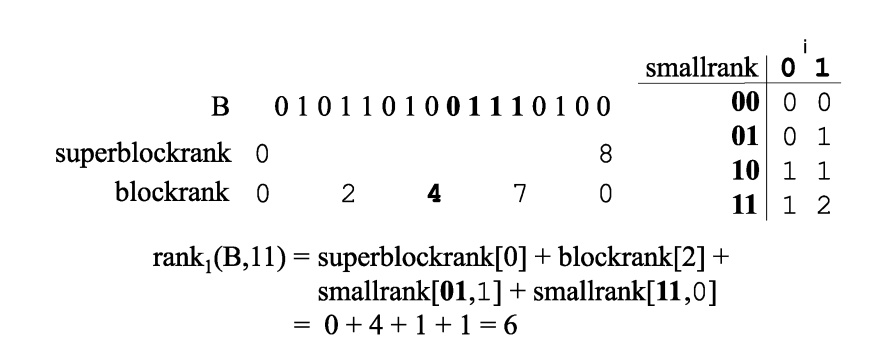
\includegraphics[width=150mm]{images/BVFastRank.png}}
\caption{Пример вычисления ранка, используя $o(n)$ дополнительной памяти}
\end{figure}
\noindent
\newpage
\subsubsection{Эффективная реализация операции $select_b(index)$}
Эффективная реализация $select_1(index)$ оказывается немного сложнее, чем операции $rank_1(pos)$. Основная проблема здесь заключается в том, что первый же ответ $select_1(index)$ может дать число от $0$, до $n$. В связи с этим здесь применяется приём разбиения блоков на длинные и короткие.

Рассмотрим упрощённую реализацию Munro and Clark \cite{clark1996efficient}. Сначала разобьём пространство аргументов $index \in [0, n)$ функции $select_1(index)$ на блоки длиной $\log^2{n}$ аргументов и построим массив ответов $superblockselect[j]$, который потребует
$\frac{n}{\log^2{n}}\log{n} = \frac{n}{\log{n}} = o(n)$ бит дополнительной памяти и будет отвечать на запрос вида $select_1({index} \log^2{n})$ за константное время.

Некоторые из этих блоков могут покрывать за раз слишком большой диапазон в $B$, поэтому нельзя хранить результаты в массиве $2\log\log n$, как это было сделано в $rank$. Чтобы обойти эту фундаментальную проблему, вводится понятие \textit{длинных} и \textit{коротких} блоков. Блок называется длинным, если он покрывает больше, чем $\log^4{n}$ позиций в $B$, остальные блоки называются короткими. Можно заметить, что количество длинных блоков не превышает $\frac{n}{\log^4{n}}$, что позволяет хранить их результат в ячейках по $\log n$ бит. В итоге длинные блоки требуют всего $\frac{n}{\log^4{n}} \log^2{n} \log n = \frac{n}{\log{n}}$ бит памяти.

Короткие блоки содержат $k = \log^2{n}$ аргументов для $select_1({index})$, результат которых покрывает не более $\log^4{n}$ позиций в массиве $B$. Чтобы уложиться снова в $o(n)$ по памяти, необходимо разделить эти блоки на миниблоки, которые отвечают за $\log^2{k} = \log^2{\log^2{n}} = O((\log \log n)^2)$ аргументов. Как и в $rank$, значения в $miniblockselect[j]$ являются относительными блока, т.е.
${select}_1(j \log^2{k}) = {miniblockselect}[j] + {superblockselect}[\frac{j \log^2{k}}{\log^2{n}}]$. Каждый результат \textit{miniblock} находится в диапазоне $[0, \log^4{n}]$, поэтому требует всего $\log \log^4{n} = 4\log\log n$ бит. Таким образом мимниблоки требуют всего $\frac{n}{\log^2{k}} \log \log^4{n} = \frac{4 n}{(2\log \log n)^2} \log \log n = O(\frac{n}{\log \log n}) = o(n)$ бит.

Теперь снова нужно разбить миниблоки на длинные и короткие. Длинные миниблоки покрывают в массиве $B$ более $\log n$ битов, все остальные минимблоки будут называться короткими. Опять же, для длинных миниблоков значения будут храниться в явном виде. Их количество не более $\frac{n}{\log n}$, а хранят они $\log^2{k}$ значений, поэтому всего длинные миниблоки занимают $O(\frac{n(\log \log n)^3}{\log n})$ бит. Для коротких миниблоков, которые покрывают не более $\log n$ бит, достаточно хранить таблицу ответов размером $O(\sqrt{n}\log{n}\log\log {n})$ бит или же на современном процессоре воспользоваться встроенной операцией $select_1$ для чисел.

В итоге получается, что ценой $o(n)$ бит дополнительной памяти можно выполнять операцию $select_1$ для всего битового массива $B$. Однако, т.к. далее эта структура данных будет применяться на внешнем носителе, операция $select$ может потребовать слишком много случайных операций ввода-вывода, поэтому в экспериментальной реализации для операции $select_1$ был сделан просто массив с ответами, который хотя и занимает $n\log{n}$ бит памяти, однако позволяет гораздо быстрее находить ответ. Операция $rank_1$ была сделана в эффективной по памяти реализации, которая описывалась в предыдущей главе.

\subsubsection{Wavelet Tree}
Естественным логическим продолжением битового массива является структура данных под названием \textit{Wavelet Tree}, построенная из набора битовых массивов. В главе про поиск подстроки в строке при помощи обратного поиска (\textit{Backward Search}) использовался массив $T^{BWT}$, который позволял на каждой итерации получить новый интервал для суффикса паттерна $P$. Однако там подразумевалось, что существует операция подсчёта количества какого-либо символа до какой-то позиции в тексте $T^{BWT}$. Как раз рассматриваемая структура данных \textit{Wavelet Tree} позволяет ответить на этот вопрос на константное время, а именно она реализует $rank_k(WT, pos)$, а также $select_k(WT, index)$, где $WT$ - Wavelet Tree.

Рассмотрим текст $T$, который составлен из алфавита размером $\sigma$. Сопоставим каждому элементу алфавита число от $0$, до $\sigma - 1$, что потребует для каждого символа $h = \lceil \log \sigma \rceil$ бит. Далее построим дерево из битовых массивов. На первом слое будет один битовый массив размером $n$, на следующим два массива, в сумме размер которых $n$, затем четыре и т.д. до $h$-ого слоя. Если символ в тексте $T[i]$ имеет старший бит 0, то в этом массиве на позици $i$ будет записан 0, иначе 1. Далее все символы со старшим битом 0 сопоставляются с левым массивом, а остальные с правым. Тогда на втором слое рассматривается более младший бит бит у символа и, также как на первом слое, если этот бит 0, то на $j$-ую позицию устанавливается 0, иначе 1. И снова у кого бит был равен 0, сопоставляются с левым следующим подслоем текущего слоя. Так повторяется $h = \log \sigma$ раз, что в итоге приводит к дереву битовых массивов, которое кодирует текст $T$ за $n \log \sigma$ бит памяти, и называется \textit{Wavelet Tree}.

Пример такого дерева для текста T="araadl\_ll\$\_bbaar\_aaaa" показан на рисунке на рис. 6. Хранятся только битовые последовательности, а тексты и переходы, которые есть на рисунке указаны исключительно в целях удобства и наглядности.

\begin{figure}[h!]
\center{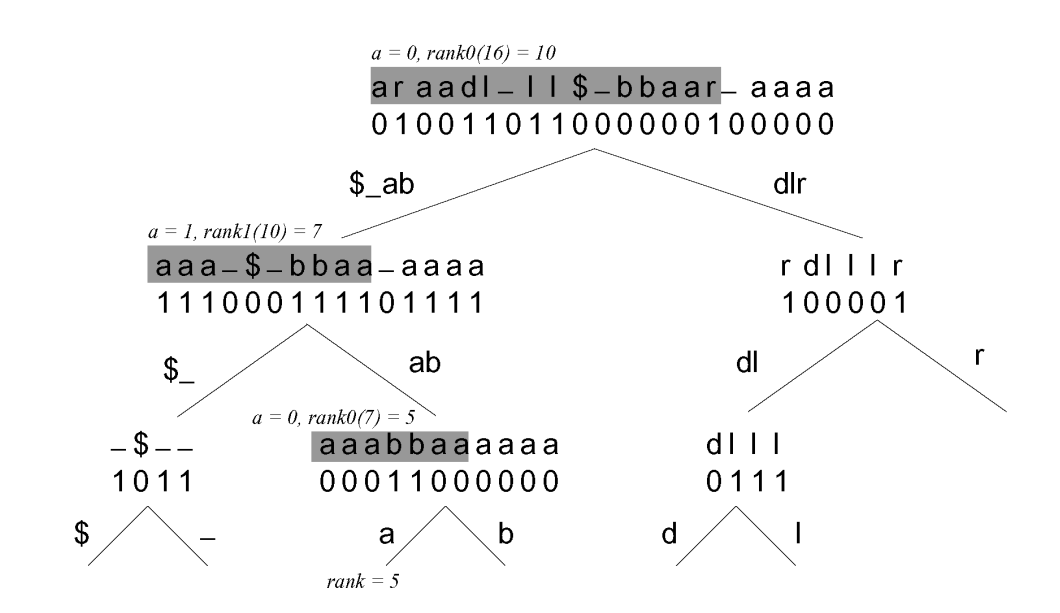
\includegraphics[width=150mm]{images/WT.png}}
\caption{Wavelet Tree}
\end{figure}
\newpage

Данная структура данных позволяет выполнять операцию ранк для любого символа из алфавита (конвертированного перед этим в число), представляя его как последовательность бит от старшего к младшему. Снова обратимся к рис.6 и рассмотрим как выполняется операция $rank_a(16)$. В данном дереве символу $a$ соответствует битовая последовательность $path = {0,1,0}$, поэтому на первом слое выполняется операция $rank_0(16) = 10$ и выбирается левый узел. В новом узле уже рассматривается следующий бит $1$, поэтому для этого массива выполняется операция $rank_1(10) = 7$ и выбирается правый дочерний узел. На последнем слое выполняется $rank_0(7) = 5$, который и вычисляет итоговый ответ $=> rank_a(16) = rank_0(B_4, rank_1(B_1, rank_0(B_0, 16))) = 5$.

С операцией $select_k(index)$, где $k \in [0, \sigma)$, всё с точностью наоборот. Сначала рассматривается самый нижний слой, для него выполняется $select_b$, затем выбирается следующий более верхний слой и т.д., пока не будет рассмотрен самый верхний слой.

Операция $get(i)$ выполняется аналогично $rank$. Сначала выполняется $j = rank_b(B_0, i)$, где $b=B_0[i]$. Затем, в зависимости от 0 или 1 выбирается левый или правый узел. Далее в новом массиве $B'$ выполняется $rank_{b'}(j)$, где $b'=B'[j]$ и так далее до последнего слоя. Тем самым получится битовая последовательность $b, b', b'', ...$, которая и определит символ, что стоял на позиции $i$ в исходном тексте $T$.

В итоге при помощи структуры \textit{Wavelet Tree} можно закодировать текст размером $n \log{\sigma}$ и занять при этом $n \log \sigma + h \cdot o(n) = n \log \sigma + o(n\log\sigma)$ дополнительной памяти, при этом получить операции $get(i)$, $rank_k(pos)$, $select_k(index)$ за константное время, где $k \in [0, \sigma)$. В данной работе самое важное для этой струткруы данных это не только умеренный размер, а быстрое время ответа на запросы типа $rank_k$ и $select_k$, что в дальнейшем будет использоваться над закодированным в WT текстом метасимволов.

\subsection{String B-Tree. Строковое дерево поиска}
После рассмотрения базовых структур данных для поиска паттерна $P$ в тексте $T$ и сжатых представлений этого текста в оперативной памяти, можно перейти от $in-memory$ к $on-disk$ структурам. $on-disk$ структуры данных представляют из себя специально спроектированные для работы с блочными устройствами \cite{cobb2012nvm} структуры, которые ориентируются, что одна единица чтения-записи в диск - это блок или страница \cite{agrawal2008design}, а время доступа и латентность кслучайной области на порядки больше, чем у \textit{RAM} оперативной памяти\cite{koo20121}. Поэтому части таких структур данных строятся и выравниваются на диске в форме блоков, чтобы аккуратно и без лишних действий их можно было записать или считать с диска.

Одной из основных on-disk структур данных является \textit{B-Tree}. B-Tree - это сильноветвящееся дерево поиска, которое хранит каждый свой узел в одном блоке, а количество потомков может быть порядка сотен. Такое представление поискового дерева позволяет за каждое блочное чтение уменьшать область поиска в два порядка, тем самым за минимальное количество операций ввода-вывода получать с диска нужные данные. Для примера рассмотрим B-Tree, у которого в одном 500 потомков, тогда уже на третьем слое будет $500^3 = 125'000'000$ индексируемых единиц. Такая структура данных применяется, например, для хранения inode в файловой системе $Ext2$ \cite{phillips2001directory}.

Чтобы обобщить идею B-Tree на строки, Paolo Ferragina и Roberto Grossi \cite{ferragina1999string} предложили и полностью описали концепцию \textit{String B-Tree} - строкового дерева поиска. Суть его в следующем. Рассмотрим текст $T[0, n-1]$ и построим над ним суффиксный массив. Затем разобьём этот массив на интервалы длиной от некоторого $b$ до $2b$. Каждый полученный интервал со всеми числами поместим в листовые узлы дерева. Пусть первый листовой узел обозначается $\sigma_0$, следующий $\sigma_1$ и т.д. Введём обозначение $L(\sigma_i)$ и $R(\sigma_i)$ для самой маленькой и самой большой строки в узле $\sigma_i$, тогда в каждом листовом узле $\sigma_i$ лежат свои строки $[L(\sigma_i),...,R(\sigma_i)]$. Следующий слой узлов String B-Tree строится из минимальных и максимальных слоёв потомков. Например, в первом внутреннем узле будет $[L(\sigma_0), R(\sigma_0),L(\sigma_1), R(\sigma_1),...,L(\sigma_{k-1}), R(\sigma_{k-1})]$, на втором $[L(\sigma_k), R(\sigma_k),L(\sigma_{k+1}), R(\sigma_{k+1}),...,L(\sigma_{y-1}), R(\sigma_{y-1})]$ и т.д. Следующий слой узлов строятся из минимальных и максимальных текущего слоя и так, пока не закончатся узлы. Количество внутренних слоёв будет составлять $\lceil \log_b{n} \rceil$, а суммарно с учётом последнего слоя $\lceil \log_b{n} \rceil + 1$. Такая структура позволяет точно определить по текущему паттерну в каких следующих узлах он будет расположен, потому что эти интервалы $[L(\sigma_0), R(\sigma_0),...,L(\sigma_{k-1}), R(\sigma_{k-1})]$ суффиксного массива непрерывны и упорядочены. Более наглядно схема внутренних узлов схематически представлена на рис.7 на примере узла $\pi$ и потомков $\sigma_1, ..., \sigma_g$.

\begin{figure}[h!]
\center{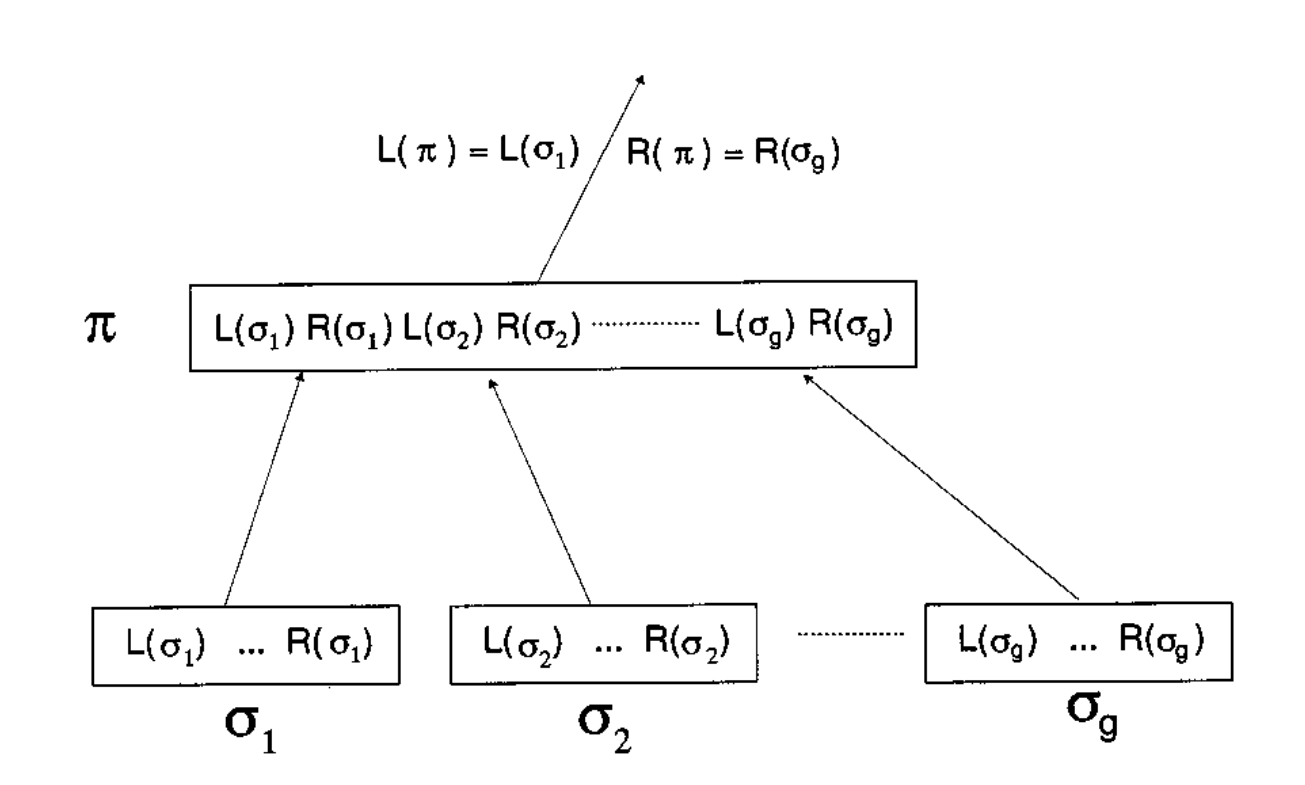
\includegraphics[width=120mm]{images/SBT_LR.png}}
\caption{Узел $\pi$ структуры String B-Tree, который хранит в себе минимальные и максимальные значения потомков $\sigma_1$, ..., $\sigma_g$}
\end{figure}

После того, как стала понятна структура узлов внутри $SBT$, необходимо рассмотреть внутреннюю структуру самих узлов. Их основная задача, как узлов поискового дерева, заключается в том, чтобы по входному паттерну $P$ с позиции $lcp$ находить позицию следующего узла дерева за эффективное время. Такую задачу решает структура данных бор или же сжатый бор - дерево, которое хранит в листьях искомые строки, в узлах разбивает строки, которые начинались с одного префикса, по отличительным буквам, а на рёбрах хранит последовательность общих символов. Однако сложность заключается в том, что каждый узел в String B-Tree обязан хранить от $b$ до $2b$ потомков (кроме корня) и при этом занимать места не более чем один блок на диске. Сжатый бор таким свойством не обладает - ему необходимо хранить рёбра, которые могут быть любой длины. Поэтому необходима структура данных, которая занимает линейное количество места и при этом требует минимальное количество обращений к диску для сравнения паттерна. Одна из таких структур - это \textit{Patricia Tree}.

\textit{Patricia Tree} можно построить из компактного бора, если на рёбрах хранить не всю общую строку, а только её первый символ, а в узлах хранить текущую общую длину (либо же $lcp$). Тогда такое дерево будет занимать линейное количество места и более того иметь предсказуемый максимальный размер, что совершенно необходимо, чтобы спроектировать и разместить его внутри блока. Такое дерево представлено на рис. 8 \cite{ferragina1999string}.

\begin{figure}[h!]
\center{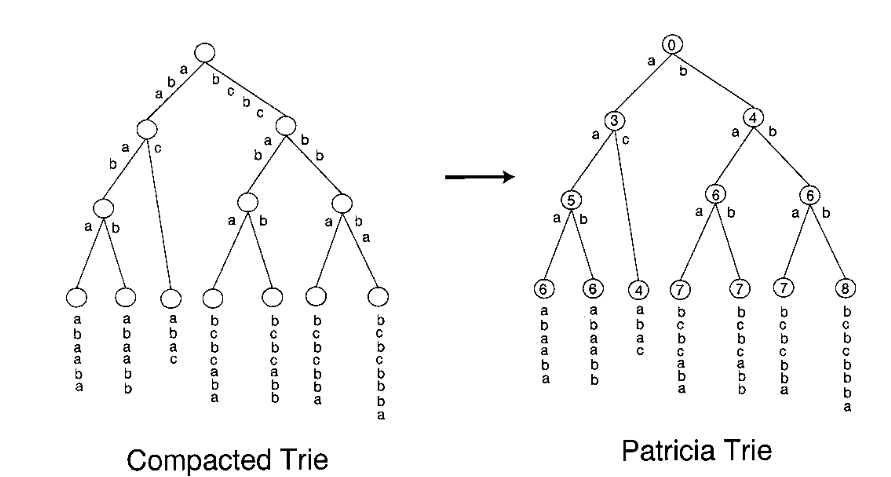
\includegraphics[width=150mm]{images/PT.png}}
\caption{Наглядное представление того, как построить дерево из сжатого бора в Patricia Tree}
\end{figure}

Поиск по такому дереву делается в две фазы и называется слепым поиском или \textit{Blind Search}. Пусть мы уже находимся на одном из внутренних узлов SBT, тогда точно известно число $lcp$ - наибольший общий префикс паттерна со всеми строками этого узла. Первая фаза заключается в том, чтобы пройтись по Patricia Tree сравнивая только одиночные буквы паттерна и узлов. Таким образом находится начальный листовой узел. Затем находим длину наибольшего общего префикса $P$ и найденного узла, учитывая, что нам уже известен входной $lcp$. После этого уже на второй фазе поднимаемся по дереву и ищем место, где произошла "ошибка" и выбираем правильное направление, которое приведёт к итоговой позиции следующего потомка или же, если это листовой узел, то к итоговой строке, а также новый $lcp$.

Для примера на рис. 9 \cite{ferragina1999string} рассматривается поиск паттерна $P=bcbabcba$ в узле $\pi$, который хранит последовательность чисел $\mathscr{I}_{\pi}$, обозначающую \newline $[L(\sigma_0), R(\sigma_0),...,L(\sigma_{k-1}), R(\sigma_{k-1})]$. Слепой поиск начинается с первой буквы паттерна $b$, затем выбирается соответствующий правый узел. Далее, т.к. в узле указано $lcp=4$, то рассматривается четвёртый символ в паттерне - $a$ и выбирается правый потомок. На этом этапе алгоритм ошибается от истинного пути, однако на втором этапе эта ошибка будет исправлена. Повторяя эту операцию алгоритм доходит до листового узла со строкой $bcbcbbba$. Затем вычисляется $lcp$ между этой строкой и паттерном $P$, получая $lcp=3$. Используя общую длину, находится позиция, где произошла ошибка (на неё указывает так называемая \textit{hit-node}), и выбирается правильное направление по символу ошибки. В данном случае $P[lcp]=a$, а у листовой ноды $S[lcp]=c$. Т.к. $a < c$, то выбирается самый левый нисходящий узел, исправляя тем самым ошибку на первой фазе\cite{ferragina1999string}.

\begin{figure}[h!]
\center{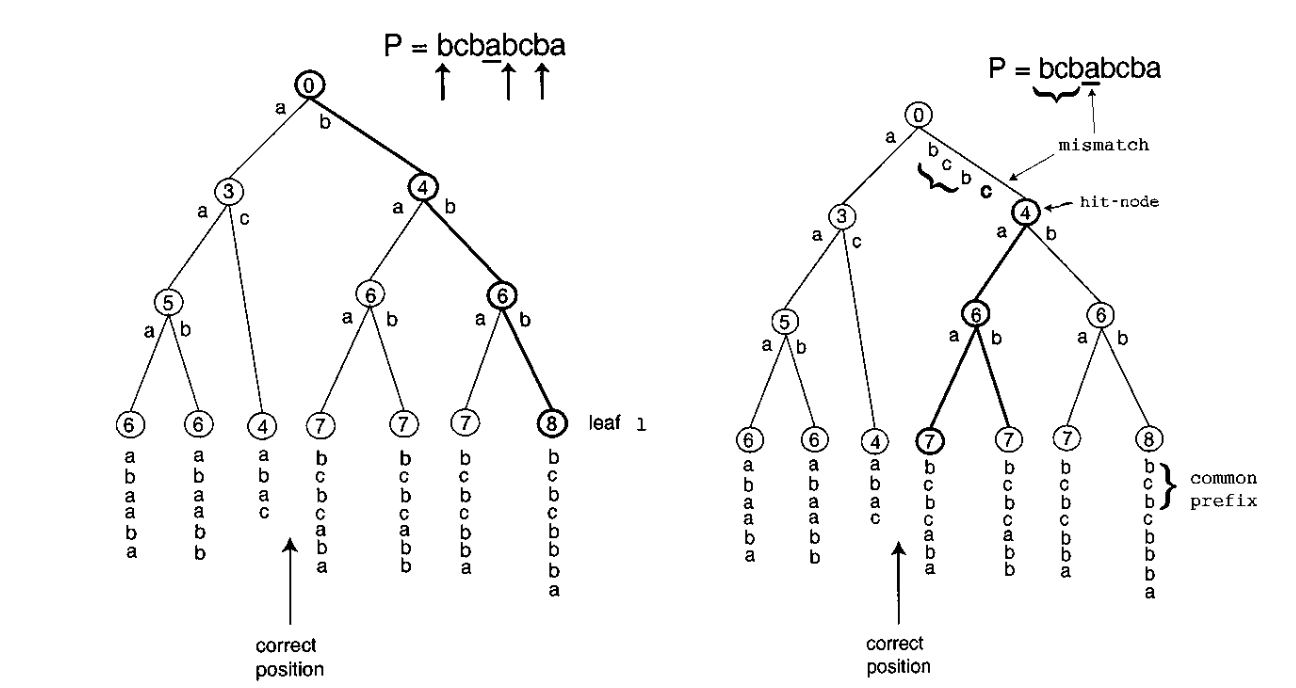
\includegraphics[width=150mm]{images/PT_Search.png}}
\caption{Поиск в Patricia Tree}
\end{figure}

Благодаря комбинации B-Tree для внешней структуры и Patricia Tree для внутренней структуры данная структура String B-Tree позволяет выполнять поиск паттерна $P[0, p-1]$ в тексте $T[0, n-1]$ за $O(\frac{p + occ}{B} + \log_BP{n})$ операций ввода-вывода диска, где $p = |P|$, $occ$ - количество найденных совпадений, $B$ - размер блока диска.

Однако, как будет показано в главе $"$Результаты эксперимента$"$, размер String B-Tree превосходит размер исходного текста в десятки раз, что может затруднить использование данной структуры данных для анализа достаточно больших последовательностей. В связи с этим возникает задача эффективной комбинации сжатых индексов и on-disk структур данных. Одна из таких структур будет рассмотрена в следующей главе.

\subsection{Geometric BWT. Геометрическое преобразование Берроуза-Уилера}
При построении String B-Tree для ветвления использовался стандартный алфавит $\Sigma$ текста $T[0,n-1]$, однако используя $BWT$ можно эффективно использовать новый алфавит, построенный из $\Sigma$. Новый взгляд на преобразование Берроуза-Уилера был дан \textit{Rahul Shah} и \textit{Wing-Kai Hon}, которое они назвали \textit{Geometric BWT - GBWT} \cite{chien2008geometric}.

Рассмотрим текст $T[0, n-1]$ и некоторое число $d = \delta \log_{\sigma}{n}$, которое будет обозначать длину метасимволов текста $T$, причём $\delta$ берётся равной $\frac{1}{4}$. Метасимволом текста $T$ будет обозначаться последовательность длины $d$ символов из исходного алфавита $\Sigma$, а текстом из метасимволов - $T'$, например, первым метасимволом будет $T'[0] = T[0]T[1]...T[d-1]$, вторым $T'[1] = T[d]T[d+1]...T[2 \cdot d-1]$ и т.д. Для простоты возьмём $n$ кратным $d$, однако это не уменьшает общности, потому что можно дополнить текст минимальным символом до кратности числу $d$. Полученные метасимволы являются лексикографически упорядоченными, т.к. состоят из упорядоченных символов $\Sigma$.

Построим над текстом $T'[0, \frac{n}{d} - 1]$ суффиксный массив $SA'[0, \frac{n}{d} - 1]$ и String B-Tree $SBT'$. Полученные структры данных уже позволяют выполнять поиск, однако в сильно ограниченной форме, когда паттерн начинается с существующей последовательности метасимволов. Чтобы улучшить этот поиск до посимвольного, необходимо ввести \textit{GBWT}.

Суть \textit{GBWT} заключается в том, что рассматривается текст $T'$ и построенный над ним суффиксный массив $SA'$. Затем над $T$ выполняется преобразование $BWT$, которое даёт $T_{BWT}^{'} = T'[SA'[i] - 1]$. И последним шагом метасимволы полученного текста заменяются на их отражённые слева направо. Например, если $T_{BWT}^{'}[0] = ACTG$, то после отражения $\overleftarrow{T_{BWT}^{'}}[0]=GTCA$. В итоге \textit{GBWT} над $T'$ - это последовательность метасимволов $\overleftarrow{T'[SA'[i] - 1]}$. Можно заметить, что $\textit{GBWT}$ - это просто $BWT$ над $T'$ с отражёнными метасимволами.

Чтобы использовать $T_{GBWT}$ для поиска, рассмотрим паттерн $P$, для простоты размер которого больше $d$. Введём понятие \textit{k-ого} смещения $P$, которое будет искать вхождения $P$ на позициях $i \mod{d} \neq 0$. Пусть $\widehat{P}$ - префикс $P$ длины $\pi = d - k + 1$, а $\Tilde{P}$ - суффикс $P$, полученный отниманием $\widehat{P}$ от $P$. Теперь отразим $\widehat{P}$ и добавим справа недостающие $k - 1$ нулевых символов, тем самым получим метасимвол длины $d$, который обозначим $c_{min}$. Если же вместо нулей добавить единицы, то получим $c_{max}$. Нетрудно понять, что все найденные символы, которые удовлетворяют префиксу паттерна, после отражения лежат между $c_{min}$ и $c_{max}$. Поэтому, если с позиции $i'$ строка совпадает с суффиксом $\Tilde{P}$, то достаточно проверить, что $c_{min} \le \overleftarrow{T'[i'-1]} \le c_{max}$. Такую проверку можно эффективно реализовать при помощи структуры данных Wavelet Tree, построенной над $T_{BWT}^{'}$ и её операций $rank_k$ и $select_k$. В этом и есть основная суть \textit{GBWT}. 

Полный алгоритм поиска $P$ следующий:
\begin{enumerate}
    \item Используя $SBT'$ найти диапазон $[l, r]$, такой что $SA'[l...r]$ - все вхождения $\Tilde{P}$ в $T'$.
    \item Построить $c_{min}$ и $c_{max}$ из $\widehat{P}$.
    \item При помощи Wavelet Tree найти все $y \in [l, r]$, такие что  $c_{min} \le T_{BWT}^{'}[y] \le c_{max}$.
    \item Получить $SA'[y]$ для всех $y$, чтобы получить ответ.
\end{enumerate}
Чтобы найти все вхождения $P$ в $T$, необходимо выполнить такую операцию для всех $k \in [2, d]$. 

При построении $SBT$ на самом нижнем слое неявно располагался суффиксный массив $SA$, который для обычного текста занимал $O(n \log n)$ памяти на диске, однако для текста из метасимволов размер будет заметно меньше, а именно $O(\frac{n}{d} \log{\frac{n}{d}})$. Стоит учесть, что к $SBT'$ также добовляется $WT'$ - Wavelet Tree из $T'$, поэтому эти структуры данных тоже будут занимать дополнительное место. Чтобы достоверно получить эффективность по занимаемому пространству и времени поиска, необходимо провести эксперимент и сравнить полученные резульаты.

\section{Проблема сравнения эффективности методов}
В исследованной литературе\cite{ferragina1999string}\cite{chien2008geometric} были подробно описаны детали реализаций и методы исследования, однако не было дано хорошего непосредственного сравнения SBT и GBWT между собой. Данная работа призвана заполнить этот пробел и убедиться в дисковой эффективности сжатой версии.

Стоит отметить, что перепроверка результатов существующих работ и создание своих реализаций исследуемых объектов, приносит пользу науки в целом, пересраховывая её от случайных ошибок и подкрепляя полученные ранее результаты. Можно привести пример, когда большая компания выпускала статью про новый современный алгоритм, который по её заявлению кратно быстрее существующих, однако после перепроверки результатов и написания собственной реализации выяснялись детали, после которых становилось понятно, что результаты компании были ошибочны \cite{wang2018building}.

Именно поэтому в данной работе автором были полностью реализованы исследуемые струткруры данных и лично проведены все необходимые эксперименты для сравнения эффективности методов.

В данном исследовании рассматриваются индексы над исходными текстами различной длины: от 1 Мбайта до 200 Мбайт. Это необходимо для исследования покомпонентного влияния отдельных частей структуры в разных граничных условиях на результаты всего экмперимента в целом. Так, ниже будет показано, что даже для текста размером в 1Мбайт, из-за особенностей реализации размер $WT$ при $d = 8$ будет 500 Мбайт, однако для текста в 200 Мбайт - всего 700 Мбайт. Также текст в 200 МБайт позволяет оценить различие в поведении двух методов при большом количестве данных, тем самым заставляя проявлять свою компактность для сжатых структур данных.

\section{Экспериментальное исследование}
Для проведения экспериментов, автором были реализованы String B-Tree и Geometric BWT, которые включают в себя такие струткруы данных, как patricia tree, суффиксный массив и битовый массив. Для каждой из приведённых структур данных были реализованы \textit{юнит} тесты, а для Patricia Tree также была реализована наивная версия без оптимизаций, для проверки корректности поведения основной версии. Исходный код программы был написан на языке программирования C++\cite{вандервуд2003шаблоны} стандарта 2020-ого года. Компиляция выполнялась компилятором \textit{gcc 11.3.0}.

Исходный код разделяется на две части: код структрур данных (\textit{SA}, \textit{SBT}, \textit{PT}, \textit{WT}, \textit{BV}) и тестов для этих структур.

Для проведения юнит тестов и дебага программы использовались помимо флагов отладки также флаги, подключающие адрес санитайзер и undefined behavior (UB) санитайзер для выявления незаметных на тестах ошибок, например выход за границы массива или же переполнение чисел. Пример такой компиляции в режиме \textit{Debug} представлен ниже:
\begin{lstlisting}[language=bash]
g++ -Wall -Wextra -fsanitize=address -fsanitize=undefined \
    -g3 -Og -std=c++20 dna.cpp
\end{lstlisting}

Для проведения экспериментов, определяющих производительность структур данных, использовался режим компиляции \textit{Release}, также в этом режиме для дополнительной надёжности компилировались и запускались \textit{юнит} тесты. Пример такой компиляции в режиме \textit{Release} представлен ниже:
\begin{lstlisting}[language=bash]
g++ -Wall -Wextra -O3 -std=c++20 dna.cpp
\end{lstlisting}

Для достижения поставленной цели и сравнения размеров и скорости полученных структур, были скомпилированны исполняемые файлы с различной длиной метасимвола $d$, который является параметром времени компиляции.

\subsection{Краткое изложение исследуемых структур}

После того, как было дано теоретическое описание двух структур данных для поиска паттерна $P$ в тексте $T$ во внешней памяти, а именно \textit{SBT} - структура данных без сжатых индексов и \textit{GBWT} - структура данных со сжатыми индексами, необходимо поставить эксперимент и проверить качественно их свойства и характеристики. Для удобства и ясности, приводится краткое описание этих структур:
\begin{enumerate}
    \item \textit{SBT} - поисковое дерево непосредственно над текстом $T$, состоящее из двух видов узлов: внутренние и листовые. Оба вида узлов внутри содержат \textit{Patricia Tree} и массив позиций текста $[L_k R_k,..,L_{k+b}R_{k+b}]$ для поиска за $O(1)$ I/O операций с диском. Также внутренние узлы хранят массив адресов на узлы детей, чтобы спускаться по дереву.
    \item \textit{GBWT} - это комбинация поискового дерева \textit{SBT'} и \textit{Wavelet Tree - WT'} над $T'$, размер которых зависит от параметра длины метасимвола $d$.
\end{enumerate}

Всего будет рассматриваться $8$ таких структур данных, которые построены с параметром $d \in [1,8]$, а именно одна \textit{SBT} - при $d = 1$ и семь \textit{GBWT} - при $d \in [2, 8]$.
Эксперименты проводятся на машине с процессором Intel i5-8300H, объёмом ОЗУ 16 Гб и диском NVMe SSD XPG GAMMIX S11 Pro. 

\subsection{Количество потомков в узле \textit{SBT}}
Первое наблюдение, которое даже не потребует запуска программы, а лишь её компиляции - это количество потомков в узлах при разном параметре $d$:

\begin{center}
\pgfplotsset{width=12.5cm,compat=newest}
\begin{tikzpicture}

\begin{axis}[
    xlabel = {$d$},
    ylabel = {$N$},
    title = {Число потомков $N$ от длины метасимвола $d$},
    legend pos = north east,
    grid = major,
    xtick = {1, 2, 3, 4, 5, 6, 7, 8},
    ytick = {238, 213, 193, 270, 238, 213}
]
\legend{внутренний узел, листовой узел}
\addplot coordinates {
    (1, 238) (2, 238) (3, 213) (4, 213) (5, 213) (6, 193) (7, 193) (8, 193)
};
\addplot coordinates {
    (1, 270) (2, 270) (3, 238) (4, 238) (5, 238) (6, 213) (7, 213) (8, 213)
};

\end{axis}
\end{tikzpicture}
\end{center}

Как и требовалось ожидать с ростом $d$ уменьшается количество потомков в узле, потому что размер узла фиксированный - 4096 байт, а размер символа в узле Patricia Tree $3 * d$ бит. Также, количество позиций на листовом узле больше, чем на внутреннем: при $d = 1$ на $32$, при $d = 3$ на $25$, при $d = 6$ на $20$.

\subsection{Размер String B-Tree и Geometric BWT от $d$}

Рассмотрим размер структуры данных $SBT$ (т.е. при $d=1$) над текстами $T$ с разной длиной. В качестве текста подаётся часть последовательности ДНК человека \textit{GRCh38.dna.chromosome.MT} длиной 1 MB, 20 MB, 100 MB и 200 MB.


\begin{center}
\pgfplotsset{width=12.5cm,compat=newest}
\begin{tikzpicture}

\begin{axis}[
    xlabel = {Размер текста в Мегабайтах},
    ylabel = {Размер SBT в Мегабайтах},
    legend pos = north west,
    grid = major
]
\addplot coordinates {
    (1, 12.72) (20, 296.54) (100, 1470) (200, 2680)
};

\end{axis}
\end{tikzpicture}
\end{center}

Можно заметить, что размер структуры в $13-14$ раз больше, чем размер исходного текста. Это и есть одна из причин, по которой $SBT$ не очень подходит для индексации больших текстов.

Рассмотрим размер структур $SBT$ и $GBWT$ при фиксированном размере текста, но при различном параметре $d \in [1,8]$. Здесь и далее будет подразумеваться, что поисковая структура $SBT'$ при $d = 1$ - это $SBT$, а при $d > 1$ - $GBWT$.

\begin{center}
\pgfplotsset{width=13.5cm, height=9cm, compat=newest}
\begin{tikzpicture}

\begin{axis}[
    xlabel = {Длина метасимвола $d$},
    ylabel = {Размер $SBT'$ в Мегабайтах},
    title = {Размер $SBT'$ при длине текста $T$ = 1МБайт},
    legend pos = north west,
    grid = major,
]

\legend{SBT, WT, Sum}

\addplot [ 
    draw = green,
    mark = triangle*, 
    mark options = { scale = 2.5, fill = green, draw = green}] coordinates {
(1, 12.72) (2, 6.36) (3, 4.82) (4, 3.62) (5, 2.89) (6, 2.70) (7, 2.32) (8, 2.03)
};

\addplot [ 
    draw = red,
    mark = *, 
    mark options = { scale = 1.5, fill = red, draw = red }] coordinates {
(1, 0.00) (2, 2.17) (3, 1.66) (4, 1.53) (5, 2.32) (6, 9.43) (7, 66.09) (8, 516.26)
};
\addplot [ 
    draw = blue,
    mark = square*, 
    mark options = { scale = 1.5, fill = blue, draw = blue }] coordinates {
    (1, 12.72) (2, 8.54) (3, 6.48) (4, 5.15) (5, 5.22) (6, 12.13) (7, 68.40) (8, 518.29)
};

\end{axis}
\end{tikzpicture}
\end{center}

\begin{center}
\pgfplotsset{width=13.5cm, height=9cm, compat=newest}
\begin{tikzpicture}

\begin{axis}[
    xlabel = {Длина метасимвола $d$},
    ylabel = {Размер $SBT'$ в Мегабайтах},
    title = {Размер $SBT'$ при длине текста $T$ = 20МБайт},
    legend pos = north west,
    grid = major,
]

\legend{SBT, WT, Sum}

\addplot [ 
    draw = green,
    mark = triangle*, 
    mark options = { scale = 2.5, fill = green, draw = green }] coordinates {
(1, 296.54) (2, 148.28) (3, 112.26) (4, 84.20) (5, 67.36) (6, 62.79) (7, 53.82) (8, 47.09)
};

\addplot [ 
    draw = red,
    mark = *, 
    mark options = { scale = 1.5, fill = red, draw = red }] coordinates {
(1, 0.00) (2, 49.62) (3, 37.00) (4, 30.97) (5, 28.44) (6, 33.54) (7, 89.05) (8, 539.32)
};
\addplot [ 
    draw = blue,
    mark = square*, 
    mark options = { scale = 1.5, fill = blue, draw = blue }] coordinates {
    (1, 296.54) (2, 197.89) (3, 149.26) (4, 115.17) (5, 95.80) (6, 96.32) (7, 142.87) (8, 586.42) 
};

\end{axis}
\end{tikzpicture}
\end{center}

\newpage

\begin{center}
\pgfplotsset{width=13.5cm,height=9cm,compat=newest}
\begin{tikzpicture}

\begin{axis}[
    xlabel = {Длина метасимвола $d$},
    ylabel = {Размер $SBT'$ в Гигабайтах},
    title = {Размер $SBT'$ при длине текста $T$ = 100МБайт},
    grid = major,
]

\legend{SBT, WT, Sum}

\addplot [ 
    draw = green,
    mark = triangle*, 
    mark options = {
        scale = 2.5, 
        fill = green, 
        draw = green
}] coordinates {
    (1, 1.47) (2, 0.73) (3, 0.55) (4, 0.42) (5, 0.33) (6, 0.31) (7, 0.27) (8, 0.23)
};

\addplot [ 
    draw = red,
    mark = *, 
    mark options = {
        scale = 1.5, 
        fill = red, 
        draw = red
}] coordinates {
    (1, 0.00) (2, 0.24) (3, 0.18) (4, 0.15) (5, 0.13) (6, 0.13) (7, 0.18) (8, 0.61)
};
\addplot [ 
    draw = blue,
    mark = square*, 
    mark options = {
        scale = 1.5, 
        fill = blue, 
        draw = blue
}] coordinates {
    (1, 1.47) (2, 0.98) (3, 0.74) (4, 0.57) (5, 0.47) (6, 0.44) (7, 0.44) (8, 0.85)
};

\end{axis}
\end{tikzpicture}
\end{center}

\begin{center}
\pgfplotsset{width=13.5cm,height=9cm,compat=newest}
\begin{tikzpicture}

\begin{axis}[
    xlabel = {Длина метасимвола $d$},
    ylabel = {Размер $SBT'$ в Гигабайтах},
    title = {Размер $SBT'$ при длине текста $T$ = 200МБайт},
    grid = major,
]
\legend{SBT, WT, Sum}

\addplot [ 
    draw = green,
    mark = triangle*, 
    mark options = {
        scale = 2.5, 
        fill = green, 
        draw = green
}] coordinates {
    (1, 2.68) (2, 1.34) (3, 1.01) (4, 0.76) (5, 0.61) (6, 0.57) (7, 0.49) (8, 0.43)
};

\addplot [ 
    draw = red,
    mark = *, 
    mark options = {
        scale = 1.5, 
        fill = red, 
        draw = red
}] coordinates {
    (1, 0.00) (2, 0.44) (3, 0.33) (4, 0.27) (5, 0.24) (6, 0.23) (7, 0.27) (8, 0.70)
};
\addplot [ 
    draw = blue,
    mark = square*, 
    mark options = {
        scale = 1.5, 
        fill = blue, 
        draw = blue
}] coordinates {
    (1, 2.68) (2, 1.78) (3, 1.34) (4, 1.03) (5, 0.85) (6, 0.79) (7, 0.76) (8, 1.13)
};

\end{axis}
\end{tikzpicture}
\end{center}

\newpage

Для наглядности на графиках представлен не только итоговый размер поисковой структуры, но и размер её компонент - $WT$ и $SBT$. Это позволяет заметить, что с ростом длины метасимвола, размер $SBT$ уменьшается, потому что количество символов, а значит и размер последнего слоя дерева, который неявно хранит в себе суффиксный массив $SA'$ уменьшается. Однако размер $WT$ при больших $d$ наоборот увеличивается, что связано с особенностями реализации $WT$ - каждый уровень $WT$ представляет из себя массив битовых векторов $BV$ в количестве $3^d$ на последнем слое, что и приводит к резкому скачку при больших $d$.

В итоге получается, что существует некоторый оптимальный по размеру структуры параметр $d$ в зависимости от размера текста, а именно для текстов с размерами 100Мбайт и 200Мбайт $d = 7$. В таком случае размер структуры для текста 100Мбайт будет составлять 440Мбайт, а для текста 200МБайт - 760 Мбайт, т.е. размер структуры всего в 4 раза больше, чем сам текст. Это гораздо более эффективно, чем просто $SBT$, для которого такой коэффициент размера составляет 13.

Также можно получить эмпирическую оценку для коэффициента $\delta$ из оригинальной статьи и сравнить его с предлагаемым авторами ($\delta = \frac{1}{4}$). Т.к. $d = \delta \log_{\sigma}{n}$, то $\delta = \frac{d}{\log_{\sigma}{n}} = \frac{8}{\log_{8}{200 * 2 ^ {20}}} \approx 0.87 \approx \frac{8}{9}$. Получилось в $3.5$ раза больше, однако стоит учесть, что этот коэффициент исходит из оптимальности по размеру, а не по скорости поиска.

\subsection{Время поиска $SBT$ и $GBWT$}
В предыдущем разделе было выявлено, что размер сжатой структуры данных $GBWT$ меньше в 4 раза чем обычной $SBT$, однако необходимо провести эксперимент и сравнить какой ценой эффективности поисковых запросов этот результат был получен.

Эксперимент включает в себя замер времени поиска первого вхождения случайного паттерна $P$ в текст $T$ для различных длин исходных текстов $[1MB, 20MB, 100MB, 200MB]$ и различных длин паттернов $|P| \in \{16, 32, 64\}$ символов. Количество запросов и как следствие размер выборки для усреднения времени определяется как $n / 35000$. Тогда для текстов $[1MB, 20MB, 100MB, 200MB]$ количество запросов будет $[24, 580, 2938, 5368]$ соответственно.

Стоит отметить важный момент, что замер производится на машине с операционной системой \textit{Linux Mint 21.1 Vera} основанной над \textit{Ubuntu 22.04 jammy}, в которой реализовано кэширование дисковых операций для существенного повышения I/O операций с дисками. Например, если провести эксперимент в первый раз, то среднее время запроса займёт $500 \mu s$, однако во второй уже $5 \mu s$.  Чтобы сбрасывать прочитанные блоки из ОЗУ, перед каждым экспериментом в терминале выполнялась команда:

\begin{lstlisting}[language=bash]
sudo bash -c "echo 1 > /proc/sys/vm/drop_caches"
\end{lstlisting}

Полученные в ходе проведения экспериментов графики представлены ниже:

\begin{center}
\pgfplotsset{width=13.5cm,height=9cm,compat=newest}
\begin{tikzpicture}

\begin{axis}[
    xlabel = {Длина метасимвола $d$},
    ylabel = {Время поиска в $\mu s$},
    title = {Время поиска в $SBT'$ при длине текста $T$ = 1МБайт},
    grid = major,
    legend pos = north west
]
\legend{$p = 16$, $p = 32$, $p = 64$}

\addplot [ 
    draw = blue,
    mark = square*, 
    mark options = { scale = 1.5, fill = blue, draw = blue }] coordinates {
(1, 300) (2, 466) (3, 486) (4, 489) (5, 581) (6, 942) (7, 1612) (8, 3861) 
};
\addplot [
    dashed,
    draw = red,
    mark = *, 
    mark options = { scale = 1.5, fill = red, draw = red }] coordinates {
(1, 344) (2, 495) (3, 554) (4, 616) (5, 723) (6, 912) (7, 2744) (8, 3608) 
};
\addplot [ 
    draw = green,
    mark = square*, 
    mark options = { scale = 1.5, fill = green, draw = green }] coordinates {
(1, 354) (2, 501) (3, 575) (4, 550) (5, 683) (6, 1029) (7, 2257) (8, 4220)
};

\end{axis}
\end{tikzpicture}
\end{center}

\begin{center}
\pgfplotsset{width=13.5cm,height=9cm,compat=newest}
\begin{tikzpicture}

\begin{axis}[
    xlabel = {Длина метасимвола $d$},
    ylabel = {Время поиска в $\mu s$},
    title = {Время поиска в $SBT'$ при длине текста $T$ = 20МБайт},
    grid = major,
    legend pos = north west
]
\legend{$p = 16$, $p = 32$, $p = 64$}

\addplot [ 
    draw = blue,
    mark = square*, 
    mark options = { scale = 1.5, fill = blue, draw = blue }] coordinates {
(1, 475) (2, 627) (3, 796) (4, 738) (5, 679) (6, 697) (7, 736) (8, 1135)
};
\addplot [
    dashed,
    draw = red,
    mark = *, 
    mark options = { scale = 1.5, fill = red, draw = red }] coordinates {
(1, 448) (2, 712) (3, 819) (4, 783) (5, 730) (6, 752) (7, 845) (8, 1136)
};
\addplot [ 
    draw = green,
    mark = square*, 
    mark options = { scale = 1.5, fill = green, draw = green }] coordinates {
(1, 522) (2, 726) (3, 848) (4, 805) (5, 735) (6, 764) (7, 830) (8, 1113)
};

\end{axis}
\end{tikzpicture}
\end{center}

\begin{center}
\pgfplotsset{width=13.5cm,height=9cm,compat=newest}
\begin{tikzpicture}

\begin{axis}[
    xlabel = {Длина метасимвола $d$},
    ylabel = {Время поиска в $\mu s$},
    title = {Время поиска в $SBT'$ при длине текста $T$ = 100МБайт},
    grid = major,
]
\legend{$p = 16$, $p = 32$, $p = 64$}

\addplot [ 
    draw = blue,
    mark = square*, 
    mark options = { scale = 1.5, fill = blue, draw = blue }] coordinates {
(1, 500) (2, 767) (3, 826) (4, 764) (5, 726) (6, 712) (7, 692) (8, 749) 
};
\addplot [
    dashed,
    draw = red,
    mark = *, 
    mark options = { scale = 1.5, fill = red, draw = red }] coordinates {
(1, 497) (2, 820) (3, 861) (4, 812) (5, 751) (6, 744) (7, 711) (8, 739) 
};
\addplot [ 
    draw = green,
    mark = square*, 
    mark options = { scale = 1.5, fill = green, draw = green }] coordinates {
(1, 513) (2, 822) (3, 900) (4, 825) (5, 751) (6, 733) (7, 689) (8, 762)
};

\end{axis}
\end{tikzpicture}
\end{center}

\begin{center}
\pgfplotsset{width=13.5cm,height=9cm,compat=newest}
\begin{tikzpicture}

\begin{axis}[
    xlabel = {Длина метасимвола $d$},
    ylabel = {Время поиска в $\mu s$},
    title = {Время поиска в $SBT'$ при длине текста $T$ = 200МБайт},
    grid = major,
    legend pos = south east
]
\legend{$p = 16$, $p = 32$, $p = 64$}

\addplot [ 
    draw = blue,
    mark = square*, 
    mark options = { scale = 1.5, fill = blue, draw = blue }] coordinates {
(1, 340) (2, 754) (3, 806) (4, 772) (5, 716) (6, 729) (7, 736) (8, 687)
};
\addplot [
    dashed,
    draw = red,
    mark = *, 
    mark options = { scale = 1.5, fill = red, draw = red }] coordinates {
(1, 504) (2, 796) (3, 869) (4, 818) (5, 733) (6, 758) (7, 778) (8, 700) 
};
\addplot [ 
    draw = green,
    mark = square*, 
    mark options = { scale = 1.5, fill = green, draw = green }] coordinates {
(1, 492) (2, 808) (3, 874) (4, 831) (5, 738) (6, 738) (7, 788) (8, 717) 
};

\end{axis}
\end{tikzpicture}
\end{center}

При рассмотрении времени поиска для текста в 1МБайт можно наглядно убедиться в природе алгоритма, что при поиске ему необходимо сделать $d$ итераций и для $d=8$ время поиска резко возрастает. Также на эксперименте подтвердилось очевидное свойство, что на каждом тексте время поиска более длинного паттерна в среднем дольше, чем поиск более короткого паттерна.

На основании графиков для 100 МБайт и 200 Мбайт можно заключить, что время поиска увеличивается приблизительно в 2 раза по сравнению с $SBT$. Для текста в 100 МБайт оптимальный параметр $GBWT$ ($d>1$) для времени поиска $d=7$, а для текста в 200 МБайт $d = 8$.

\section{Выводы}
В ходе проведённых экспериментов было получено, что сжатая структура данных $GBWT$ на больших текстах занимает меньше места чем $SBT$, однако уступает по скорости поиска. Различие в скорости между $d=7$ и $d=8$ несущественно, а различие в занимаемом объёме большое: при $d = 7$ для текстов длиной 100 Мбайт и 200 Мбайт размер структуры в $4.4$ и $3.8$ раз больше текста соответственно, а при $d = 8$ - в $8.5$ и $5.6$. Поэтому автором предлагается выбрать для оптимальный с точки зрения занимаемого места \underline{и} и времени поиска параметр длины метасимвола $d = 7$. При таком значении $d$ исследуемая реализация $GBWT$ имеет следующие характеристики:
\begin{itemize}
    \item Ёмкость внутреннего узла SBT 193
    \item Ёмкость листового узла SBT 213
    \item Размер структуры в $4$ раза больше размера текста
    \item Время поиска $700 \mu s$ в $2$ раза больше, чем время поиска в $SBT$
\end{itemize}

Полученные в работе результаты показали, что сжатая структура данных $GBWT$ занимает на диске в 4 раза меньше места по сравнению с несжатой версией $SBT$, ценой времени поиска, которая увеличивается в 2 раза. В ходе эксперимента, также было замечено значительное влияние кэширования уже прочитанных страниц, уменьшающее время доступа к блоку диска в 100 раз (с $500 \mu s$ до $5\mu s$), от которого приходилось явно избавляться.

Эксперимент показал, что влияние параметра $d \in [2,8]$ на время поиска для больших текстов мало, однако этот параметр сильно влияет на размер итоговой структуры, и более того существует ярко выраженный минимум размера $GBWT$ от $d$, который позволяет подобрать оптимальный для конкретной задачи параметр $d$.

Также было получено, что параметр $\delta$, приведённый в литературе в формуле длины метасимвола $d = \delta \log_{\sigma}{n}$, равный $1/4$ отличается от полученного в эксперименте: $\delta_{эксп} = 8 / 9$. Количество причин этому может быть большим, начиня с различной реализации Patricia Tree внутри узла SBT, заканчивая иной реализацией $WT$ для последнего шага поиска паттерна.

\section{Заключение}

В результате проделанной работы были исследованы и реализованы две существующие структуры данных для поиска подстроки в строке с использованием внешней памяти \textit{String B-Tree} и \textit{GBWT = String B-Tree(d) + Wavelet Tree(d)}. На эксперименте были проанализированы их преимущества и недостатки этих подходов и получены качественные результаты их размеров и времени поиска. Было подтверждено на собственной реализации, что занимаемое место сжатой струткры данных оказывается меньше исходной, что в свою очередь ещё раз подчеркнуло полезность сжатых индексов во внешней памяти.

Для больших текстов четырёхкратное уменьшение размера индекса при использовании GBWT(d = 7) вместо SBT может быть крайне полезным и полностью невелировать факт небольшого увеличения времени поиска, как следствие это приводит к актуальности $GBWT$ в ряде приложений, в которых сталкиваются с большими объёмами данных. К примеру, в области биоинформатики для анализа геномов с целью определения общих признаков заболевших исследуются файлы размером в 350 Гбайт \cite{1000HumanGenom}, которые в случае индексирования с использованием SBT потребовали бы примерно $350$Гбайт$ * 13 = 4.5$Тбайт дискового пространства, а в случае индексирования с использованием GBWT всего $350$Гбайт$ * 4 = 1.4$Тбайт, что значительно меньше. Такое существенное уменьшение занимаемых объёмов позволяет хранить большое количество данных без использования серверов, что в свою очередь может быть крайне полезным для пользователей персональных компьютеров. Также данное исследование полезно не только в области биоинформатики, но и всем отраслям, где встречается анализ больших последовательностей данных, включая анализ сигналов и поиск по тексту.

В данной работе было показано преимущество сжатой структуры данных, однако в данном направлении можно сделать ряд сравнений и исследований, чтобы сделать шаг в область улучшения полученных результатов, например:
\begin{itemize}
    \item Реализовать \textit{Wavelet Tree} не через набор \textit{Bit Vector}-ов, а через битовую матрицу.
    \item Реализовать внутреннее представление узла $SBT$ с использованием сжатых структур данных, чтобы увеличить плотность количества потомков на один узел.
    \item Представить неявно получающийся на последнем слое $SBT$ суффиксный массив позиций в тексте более ёмко, используя сжатые структуры, например, $WT$.
\end{itemize}

Область исследования сжатых структур данных во внешней памяти крайне обширна. В данной работе была затронута только её малая часть - время поиска и занимаемый размер, однако существует также задачи времени построения таких структур данных и необходимых ресурсов для этого.

\newpage
\section{Список используемой литературы}
\bibliographystyle{utf8gost705u} %% стилевой файл для оформления по ГОСТу
\bibliography{biblio} %% имя библиографической базы (bib-файла)

\end{document}
